% We mix and match units freely - day, h, ks. 
% I suggest we pick just one, e.g. write everything in ks.

% Mackenna notes on rewrite
% - not entirely sure what to do with the structure now. I split results & Discussion into SU and AB Aur subsections. Should I do that for everthing? Or do we want a larger structure change?
% - 

% Moritz notes while reading this. we'll talk about it
% DONE - Wow, you use big bin. 15 cts/bin will do - and probably give us better abundances.
% DONE - Fig 1 and 2 look nice. I wonder if that should be one figures with two panels.
% Section 4.2 needs a general description of what model we use and why before we discuss the numbers.
% I'm afraid the signal in the triplets is so low that we should probably summarize all that into just one sentence that says: We tried, but the singal is too low.
% Tab 3 needs errors if we keep it, also the units are wrong. Flux is not in photons, it woudl be photons/s/cm^2 or something like that.
% DONE - Can we get constraints on N_H from the Lya/Lyb ratios? That would be useful to help with the components.
% Long-term stability is amazing and different to what Steven saw.
% Why is it different?
% Do we want to bring in more people to help with the interpretation?
% Does the Ha lines up with the X-rays in some way? E.g. can the Ha tell us if the absorption was strong during that time or not?
% DONE? - Can we formally show that two abs components are beter than one?
% Can we formally show that the medium plasma is part of the higher abs component?

% DONE, I don't think the plot is useful - Add a comparison of different models. Include plot w/ one dataset and several models

\documentclass[twocolumn]{aastex631}

\newcommand{\vdag}{(v)^\dagger}
\newcommand\aastex{AAS\TeX}
\newcommand\latex{La\TeX}
\newcommand\apx{\ensuremath{\sim}}
\newcommand\citeeg[1]{\csitep[\emph{e.g.},][]{#1}}
\renewcommand\deg{\ensuremath{^\circ}}
\newcommand\dm[1]{\ensuremath{{\rm DM}_{\rm #1}}}
\newcommand\dmu{cm$^{-3}$~pc}
\newcommand\dt{\ensuremath{{\Delta t}}}
\newcommand\eg{\emph{e.g.}}
\newcommand\etal{\emph{et~al.}}
\newcommand\halpha{\ensuremath{{\text{H}\alpha}}}
\newcommand{\lya}{Ly$\alpha$}
\newcommand\ie{\emph{i.e.}}
\newcommand\msun{\ensuremath{\text{M}_\odot}}
\newcommand\speclum{erg~s$^{-1}$~Hz$^{-1}$}
\newcommand\todo[1]{\textcolor{red}{#1}}
\newcommand\ujy{$\mu$Jy}
\newcommand\ujybm{$\mu$Jy/bm}
\newcommand{\mps}{m\,s$^{-1}$}
\newcommand{\kepler}{{\it Kepler}}
\newcommand{\logg}{$log~g$ }
\newcommand{\metal}{[M/H]}
\newcommand{\av}{$A_V$}
\newcommand{\um}{$\mu$m}
\newcommand{\fbol}{$F_{\mathrm{bol}}$}
\newcommand{\mbol}{$m_{\mathrm{bol}}$}
\newcommand{\Mbol}{$M_{\mathrm{bol}}$}
\newcommand{\rapsq}{$R_{ap}^2$}
\newcommand{\rchisq}{$\chi^2_{\nu}$}
\newcommand{\teff}{\ensuremath{T_{\text{eff}}}}
\newcommand\kms{km~s$^{-1}$}
\newcommand{\ms}{m~s$^{-1}$}
\newcommand{\re}{$R_{\oplus}$}
\newcommand{\gaia}{\textit{Gaia}}
\newcommand{\banyan}{\texttt{BANYAN $\Sigma$}}
\newcommand{\xmm}{XMM-\textit{Newton}}
% My commands
\newcommand{\XXX}{\textit{\textcolor{red}{XXX}}}
\newcommand{\citesomething}[1]{\textcolor{red}{(cite#1)}}
\newcommand{\bluhbluh}[1]{\textit{\textcolor{red}{bluh bluh bluh(#1)}}}
\newcommand{\red}[1]{\textcolor{red}{#1}}


\begin{document}

\title{}

% Authors removed for Dual Anoymous
\correspondingauthor{Mackenna Wood}
\email{woodml@mit.edu}

%%
\author[0000-0001-7336-7725]{Mackenna L. Wood}%
\affiliation{MIT Kavli Institute for Astrophysics and Space Research Massachusetts Institute of Technology, Cambridge, MA 02139, USA}

%% 
\author[0000-0003-3654-1602]{Hans M. Gunther}%
\affiliation{MIT Kavli Institute for Astrophysics and Space Research Massachusetts Institute of Technology, Cambridge, MA 02139, USA}

\begin{abstract}
We present new XMM-Newton observations of classical T-Tauri star SU Auriga, a member of the 4 Myr old Upper Scorpius star forming region. SU Aur is a G2 spectral class star, hosting a highly inclined, dusty disk. Our data show an X-ray flare at the end of the observing period. We model the spectra using XSPEC models and measure the stellar abundances. Our results suggest a two-absorption component model provides the best fit to the data, indicating absorption by both the disk and the stellar corona.
\end{abstract}

\keywords{Young Stars, X-Ray, XMM-Newton}

% - - - - - - - - - - - - - - - - - - - - - - - - - - - - - - - - - - - - - - - - - - - - - - - 
\section{Introduction} \label{sec:intro}

%This paper discusses the X-ray emission from a young, solar-type star over a ten year period of time.  The introduction needs to cover \textbf{what big-picture information we can get from studying T-Tauri stars}, \textbf{what T-Tauri stars are}, what we know about the causes of \textbf{X-ray emission from T-Tauri stars}, and \textbf{previous long-term observations of T-Tauri stars} (X-ray and optical?).



% Why is the study of T-Tauri stars important?
Observations of young stars provide critical insight into the formation and early evolution of stars and planets. The first several million years of a star's existence are especially interesting as stars and planets undergo significant changes during that period which determine the future habitability of that system. This can help us answer questions about how our own Sun formed and how Earth became suitable to host life. Potentially even more interestingly, this can help us to understand the likelihood that other stars and planets in our galaxy similarly host life. 

% What is a T-Tauri star?
Young stars with similar masses as the sun, and smaller are known as T-Tauri stars. Specifically, this term refers to young ($< 10$ Myr), low mass ($< 3\msun$) pre-main sequence stars which exhibit \halpha emission. T-Tauri stars are typically divided into two categories, Classical T-Tauri stars (CTTS), which exhibit strong emission and significant IR and UV excess due to accretion from a circumstellar disk , and Weak-Lined T-Tauri stars (WTTS), which have much weaker \halpha{} emission and IR/UV excess \citesomething{}. The HerbigAeBe (HAeBe) stars are the more massive counterparts of CTTS with spectral types A and B. Unlike CTTS, they are not expected to form a convective envelope, and thus should not develop a strong magentic field to channel an accretion column, but primordial fields or small surface dynamos might exist.

% What do we know about T-Tauri star X-ray emission?
T-Tauri stars exhibit strong X-ray emission, emitted by both the magnetic coronae, similar to MS stars \citep[e.g. review by][]{gudel_x-ray_2009}, and accretion shocks from infalling material \citep[e.g.][]{edwards_spectroscopic_1994}. 

There is abundant observational evidence for coronae with characteristic temperatures $0.1-10$keV \citep{preibisch_evolution_2005} from these objects, with strong continuum emission as well as emission lines. In addition to the coronae, accretion shocks with characteristic temperatures of $\sim0.3$keV can occur when the star's magnetic field funnels material from the surrounding accretion disk onto the stellar surface. 

\red{HMG: I'm just adding pieces right now, we probably want to move them around in order later.}

Due to the interstellar mass function, there are only few HAeBes (the most prominent are \object{AB Aur} and \object{HD 163296}) within 150~pc of the sun, both have been extensively studied. Both are surrounded by disks that can be imaged and likely contain planets \citep[e.g.][]{2023ApJ...957...11D,2024arXiv241011939D} and that show gaps and features compatible with planet formation. Many HAeBes show X-ray activity pointing to sufficient magnetic fields \citep{2023MNRAS.521.2427R,2024MNRAS.530.3020A}, though it is unclear how those fields are powered. HD~163296 is also the source of a well-collimated jet, which consists of several layers with the innermost layer reaching a few hundred km~s$^{-1}$ and travelling shock waves in that jet are strong enough to be seen in the UV and in X-ray emission \citep[][and references therein]{2013A&A...552A.142G}. No such jet has been found in AB Aur, which could be due to differences in recent accretion history or structural differences in the magnetic field such that AB~Aur is not able to collimate its outflow in the same way. On the other hand, \cite{telleschi_first_2007} observed hints of rotational modulation in the X-ray lightcurve of AB~Aur, indicating a spot (magnetic or accretion) on the surface of the star that rotates in and out of view as typically seen on coronally active cool stars.

% Tie this back to the why-do-we-care message in the first paragraph
X-rays can penetrate deeply into the disks and influence the chemistry of grain formation \citep[review by][]{2000prpl.conf..429G} and drive the timescaled of planet formation \citep[see review by][]{2014prpl.conf..475A}, so understanding the properties and the ultimate power sources of the high-energy radiation in CTTS and HAeBes is required to understand the pathways of planet-formation. Of course, planets from over millions of years, while a single X-ray observations often only lasts for hours and we know that active stars show variability on a wide range of time scales. Only now can we begin to track X-ray properties of CTTS and HAeBes over many years or decades and results begin to trickle in. 

% What have long-term observations told us about T-Tauri coronae & coronal stability?
In the eponymous CTTS T~Tau \citet{schneider_multiepoch_2018} find X-ray variability of about a factor of two, both within observations and also over longer time periods; in all cases the X-ray emission is coronally dominated. An opposite case is TW~Hya, which has also be targets by grating spectroscopy for several years, but shows accretion-domintaed spectra in all cases \citep{2009A&A...505..755R,2012ApJ...760L..21B}.
\citet{silverberg_stable_2023} found that the cool component of young binary XZ Tau was steady over a $\sim 20 yr$ period, while the hot component varied.

% I've moved that up.
% Introduction to Herbig AB stars
%At slightly higher masses than T Tauri stars, Herbig AB stars are those young stars with masses just greater than the sun. 

% 

% Paper summary
In this paper we analyze two epochs of X-ray observations separated by about a decade for the cTTs SU Aur and the Herbig AB star AB Aur. We model the global spectra and the high-resolution RGS spectra using models to determine plasma properties and abundances for each. We provide an overview of the stellar properties of SU Aur in Section \ref{sec:star}. In Section \ref{sec:observations} we describe the observations and reduction. We discuss the results of the spectral fitting, and the light curve and optical spectroscopy analysis in Section \ref{sec:results}. Lastly, we conclude with a discussion in Section \ref{sec:discussion}.

% - - - - - - - - - - - - - - - - - - - - - - - - - - - - - - - - - - - - - - - - - - - - - - - 
\section{Stellar Properties} \label{sec:star}

\subsection{SU Aur}
SU Aur (= HD 282624), is a G2 spectral class, classical T Tauri star. It is a member of the Taurus-Auriga star forming region, and is 4 Myr old \citep[e.g.][]{dewarf_intrinsic_2003}. It forms a proper-motion pair with the nearby Herbig Ae star AB Aur \citep{dewarf_intrinsic_2003}, which is separated by $3.11'$ on the sky.

Given SU Aur's proximity and brightness compared to similar T-Tauri stars, it has been extensively observed over $30+$ years in a range of wavelength regimes \citep[e.g.][]{giampapa_synoptic_1993, dewarf_intrinsic_2003, robrade_xmm-newton_2006, labdon_dusty_2019, labdon_imaging_2023}, \red{identifying numerous interesting features.} Like other cTTs, SU Aur has a dusty, highly inclined accretion disk \citep{akeson_observations_2005, labdon_dusty_2019, labdon_imaging_2023}, prominent, variable \halpha{} emission \citep[e.g.][]{giampapa_synoptic_1993}, optical variability including flares \citesomething{} and dimming events of up to $1$ magnitude \citep[e.g.][]{dewarf_stromgren_1998, grankin_su_aur_2018}, rapid stellar rotation \citep[e.g.][]{giampapa_synoptic_1993, unruh_multisite_2004}, and strong X-ray emission with a soft excess \citesomething{}. We list observed and measured properties of SU Aur in Table \ref{table:su_aur_properties}. 
    
\begin{table}[ht!]
    \centering
    \begin{tabular}{|l|c|c|}
    \hline
    Property & Value & Reference \\
    \hline
    \multicolumn{3}{|c|}{Stellar Properties}\\
    \hline
    SpT & G2 III & \cite{dewarf_intrinsic_2003} \\
    \teff (K) & 5550 & \cite{dewarf_intrinsic_2003} \\ 
    $R_*$ ($R_\odot$) & $2.61^{0.20}_{-0.23}$ & \cite{dewarf_intrinsic_2003} \\
    $M_*$ ($M_\odot$) & $2.0 \pm 0.1 $ & \cite{dewarf_intrinsic_2003} \\
    Age (Myr) & $4 \pm 1$ & \cite{dewarf_intrinsic_2003}\\
    d (pc) & $156.986 \pm 0.7467$ & Gaia DR3\\
    $L_{bol}$ & & \\
    $L_x (10^{30} erg s^-{1})$ & 3.7 & ROSAT \\
    $A_V$ & & \\
    $vsin(i)$ (km/s) & $59\pm2$ & \citet{nguyen_close_2012} \\
    \hline
    \multicolumn{3}{|c|}{Disk Properties} \\
    \hline
    $i$ (\deg) & $56.9 \pm 0.4$ & \cite{labdon_imaging_2023} \\
    $R_{inner}$ (AU) & 0.16 & \cite{labdon_imaging_2023} \\
    \hline   
    \end{tabular}
    \caption{Stellar Properties of SU Aur.}
    \label{table:su_aur_properties}
\end{table}

\subsection{AB Aur}
AB Aur, HD 31293, is a A0 spectral class, Herbig Ae star. It is a member of the Taurus-Auriga star forming region, and is 4 Myr old \citep[e.g.][]{dewarf_intrinsic_2003}.

Like SU Aur, AB Aur has been extensively observed over a broad range of wavelengths. This  allowed the identification and characterization of a complex spiral-patterned protoplanetary disk \citep[e.g.][]{fukagawa_spiral_2004, pietu_sub_arcsec_2005, tang_circumstellar_2012}, with two potential protoplanet candidates \cite{boccaletti_possible_2020, jorquera_large_2022}. \red{potentially add some more details here.}

\begin{table}[ht!]
    \centering
    \begin{tabular}{|l|c|c|}
    \hline
    Property & Value & Reference \\
    \hline
    \multicolumn{3}{|c|}{Stellar Properties}\\
    \hline
    SpT                 & A0 V &  \\
    \teff (K)           & 9500 & \citesomething{Natta et al. 2001} \\ 
    $R_*$ ($R_\odot$)   & $2.7$ & \cite{dewarf_intrinsic_2003} \\
    $M_*$ ($M_\odot$)   & $2.4 \pm 0.2 $ & \cite{dewarf_intrinsic_2003} \\
    Age (Myr)           & $4 \pm 1$ & \cite{dewarf_intrinsic_2003}\\
    d (pc)              & $155.94 \pm 0.9$ & Gaia DR3\\
    $L_{bol}$           & & \\
    $L_x (10^{30} erg s^-{1})$ &  &  \\
    $A_V$               & & \\
    $vsin(i)$ (km/s)    & $59\pm2$ & \citet{nguyen_close_2012} \\
    \hline
    \multicolumn{3}{|c|}{Disk Properties} \\
    \hline
    $i$ (\deg) & $30\pm5$ & \citet{fukagawa_spiral_2004} \\
    $R_{inner}$ (AU) & $\sim 70$ &  \\
    $R_{outer}$ (AU) & $580$ & \citet{fukagawa_spiral_2004} \\
    \hline   
    \end{tabular}
    \caption{Stellar Properties of AB Aur.}
    \label{table:ab_aur_properties}
\end{table}

% - - - - - - - - - - - - - - - - - - - - - - - - - - - - - - - - - - - - - - - - - - - - - - - 
\section{Observations} \label{sec:observations}

We used archival and new observations from \xmm{} combined with simultaneous and near-simultaneous optical photometry and spectroscopy.

\subsection{XMM-Newton Observations}

SU Aur and AB Aur have been observed with \xmm{} twice, once in 2002 (Obs ID 0101440801), and again in 2012 (Obs ID 0671960101). In both cases, both SU Aur and its co-moving companion AB Aur were visible in the field. The 2002 data has been previously analyzed by \citet{robrade_xmm-newton_2006} and \citet{franciosini_xmm-newton_2007}.

We uniformly reduced all data using the standard \xmm{} Science Analysis System (SAS) software, version 21.0. 

Following standard practice, we selected a good time interval with a total count rate $<0.35 \mathrm{ct}\;\mathrm{s}^{-1}$ to remove a background flare. Data were then processed using the standard scripts, \texttt{epproc}, \texttt{emproc}, and \texttt{rgsproc}.

% EPIC
The spectra and lightcurves from the MOS and PN were extracted from a circular region centered on the target. \red{We set the extraction radii for the spectra and lightcurves to $800$ pixels and $600$ pixels for SU Aur and AB Aur, respectively.} We background-corrected using background spectra and lightcurves extracted from a large, apparently source-free region on the same chip. The soft and hard lightcurves were extracted separately, soft from $0.2 - 1.5$~keV, and hard from $1.5 - 10$~keV. The MOS and PN lightcurves were combined using \texttt{elcbuild} and are shown in Figures \ref{fig:su_aur_lc} and \ref{fig:ab_aur_lc}. 

For each epoch, we extracted spectra using two different time intervals to separate the quiescent and flaring data. This time was selected such that the flare rise phase is included in the extracted flare spectrum (see \ref{sec:su_aur_flare}). 

% RGS
To reduce the background in the RGS spectra, we limited the extraction region to 75\% of the PSF. We then combined the data from RGS 1 \& 2 using the \texttt{rgscombine} script. \red{Given the low count number, the RGS data is not separated into flare and out-of-flare phases}. % Is that important?
% OM
We extracted the OM data using the fast chain processing script, \texttt{omfchain}.

% - - - - - - - - - - - - - - - - - - - - - - - - - - -
\subsubsection{Obs 0101440801}
Obs 0101440801 started at $MJD = 52173$ with a total observing time of $130$~ks. Neither EPIC PN nor the OM were active for these observations.
We followed the data processing steps described above.

% SU Aur Flaring
SU Aur has three visible periods of activity, the first of which is the longest and brightest (see Figure \ref{fig:su_aur_lc}, top panel), and we extract that one separately, treating the remainder of the spectrum as ``quiescent''. At the beginning of the observation, SU Aur is in an elevated flux state, with a flare shortly after the start. Therefore, we consider the first part of the observation to be the flaring interval, ending at $MJD = 52173.3287$, and the remainder of the observation to be quiescent.

% AB Aur Flaring
AB Aur has no visible flares in this observation, and the full time interval is taken to be quiescent.

% - - - - - - - - - - - - - - - - - - - - - - - - - - -
\subsubsection{Obs 0671960101}  % 2012
Obs 0671960101 started at $MJD = 55973$ with a total observing time of $103$~ks. The EPIC MOS, EPIC PN, and RGS cameras were operational, with the OM operational for the first half of the observation period. 

There is a single flare in SU Aur, visible at the end of the observation period. We select the data from before $MJD=55973.9305$ as the quiescent data, and the data after $MJD=55973.9305$ for the flaring time interval.

There are no visible flares in AB Aur during this observation. 

% - - - - - - - - - - - - - - - - - - - - - - - - - - - - - - - - - - - - - - - - - - - - - - - 
\subsection{Optical Observations}

% Right now I'm only using the optical spectra from the ARAS group.
% There is a lot more optical data (photometry + spectroscopy), but I'm not using it currently.

Optical observations taken by the ARAS group\footnote{\url{https://aras-database.github.io/database/about.html}} were planned to coincide with the 2012 XMM-Newton observations. A total of $13$ spectra were taken by three observers. One observation was taken using a LISA spectrograph, providing a resolving power of $\sim800$, significantly lower than the other observations, and was not included in the analysis. The other $12$ observations were all taken using an ATIK 314 L+ camera. Eight of the observations were taken using a LHIRES III grating with 1200l/mm and a $D=0.41$~m telescope, providing a resolving power of $R\sim5000$. The other four were taken with a LHIRES III grating with 600l/mm, on a $D=0.28$~m telescope and a $D=0.085$~m refractory telescope, providing resolving power of $R\sim3400$ and $R\sim4400-4700$, respectively. 



\section{Results}\label{sec:results}
% - - - - - - - - - - - - - - - - - - - - - - - - - - - - - - - - - - - - - - - - - - - - - - - 
We first discuss results for SU Aur in Section \ref{sec:su_aur} and then for AB Aur in Section \ref{sec:ab_aur}. We discuss lightcurves and spectra for both targets. All spectral analysis is done with the Sherpa software \citep{burke_sherpasherpa_2024}; plasma emission is described by APEC models \citep{foster_updated_2012}. All fit uncertainties are listed at the $1\sigma$ level.  For all fits we use the solar abundance scale from \citet{asplund_chemical_2009}.

\subsection{SU Aur} \label{sec:su_aur}

\subsubsection{X-Ray Lightcurve} \label{sec:lightcurve}

The X-ray lightcurves from 2002 and 2012 are shown in Figure \ref{fig:su_aur_lc}. In 2002, the observation begins in an elevated state, likely a flare, that decays about 4~h into the observation. During the period, the hard flux is more enhanced than the soft flux, compared to the quiescent state. There are two shorter flux increases later on in the observation, and in both cases the hard lightcurve varies more than the soft lightcurve, consistent with magnetic activity. In 2012, most of the observation is taken up with a very smooth rise and decay of the X-ray flux from about 1.8 to 3~counts~s$^{-1}$. There is a short gap in the lightcurve in the middle of the observation due to a background flare, but the variability seen in Figure \ref{fig:su_aur_lc} is intrinsic to the source. A flare is seen towards the end of the observation, where the total count rate increases by a factor of 2.5 over $0.44$~h , followed by a short plateau of $0.9$ h and decay. The observation ends before the flux level has decayed back down to the previous level. 

\begin{figure*}[b]
    \centering
    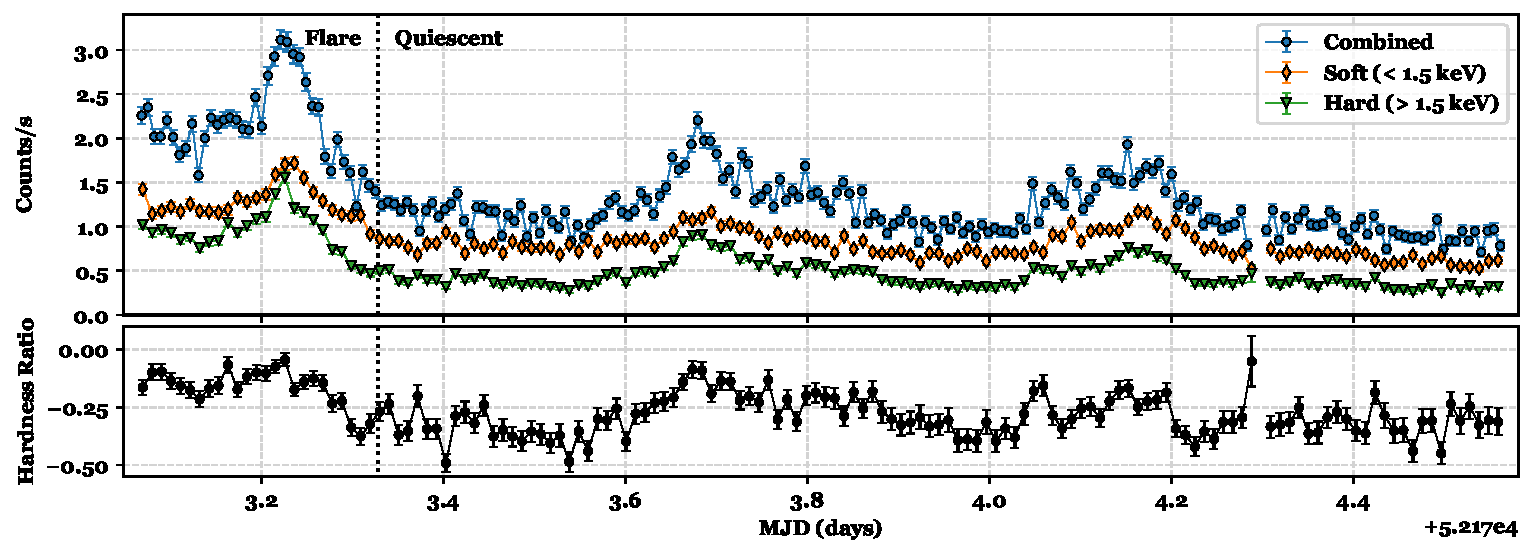
\includegraphics[width=0.9\linewidth]{Figures/SU Aur/figure_2002_lc.pdf}
    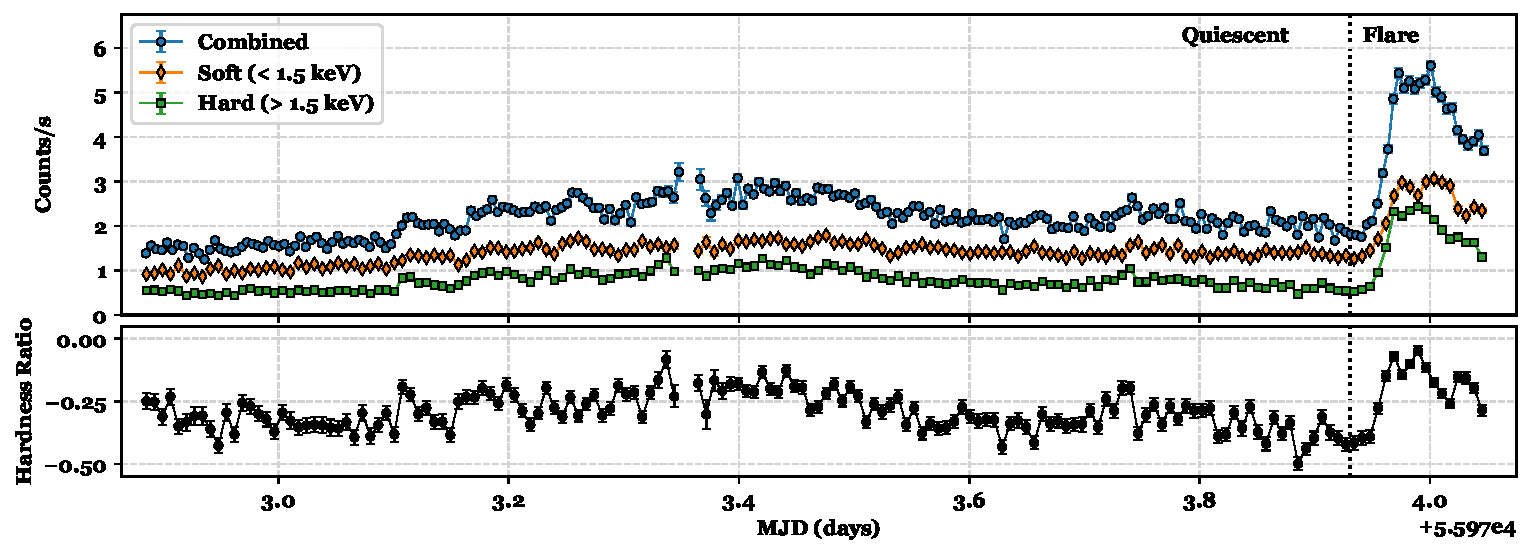
\includegraphics[width=0.9\linewidth]{Figures/SU Aur/figure_2012_lc.pdf}
    \caption{SU Aur Lightcurves. Top) EPIC LC's for 2002 data, binned to 600s intervals. Bottom) EPIC LC's for 2012 data, binned to 400s intervals. In both, the combined, soft, and hard LC's are shown, in blue circles, orange diamonds, and green squares respectively. Dotted black lines show the times at which we split the data into the flare and quiescent time intervals for each.}
    \label{fig:su_aur_lc}
\end{figure*}

% - - - - - - - - - - - - - - - - - - - - - - - - - - - - - - - - - - - - - - - - - - - - - - - 
\subsubsection{Plasma Properties} \label{sec:plasma}

To determine the plasma properties we performed spectral fitting using both the EPIC spectra and the high-resolution RGS spectra. We perform a global fit to the full spectra, and separately measure the flux in specific emission lines in the RGS spectrum. The EPIC spectra were binned to bins of 20~counts per bin. Since the absolute abundance is difficult to constrain without well-exposed grating spectra, we essentially measure relative abundances of metals. For simplicity, we fixed the Oxygen abundance to solar, allowing all other abundance values to vary. Elements with similar first-ionization potential (FIP) values were grouped and fit together, so that C, N, and O were tied (and fixed to our solar reference), Mg and Ni were tied, Fe, Ca and Al.

We attempted to obtain temperature and density diagnostics from the O and Ne He-like triplets, but found that the signal in the triplets was too low to obtain significant results.

% Model Choice
We test several different models of increasing complexity starting from a single absorption component with two temperature components (Model A). The next model, following \citet{robrade_xmm-newton_2006}, was a single absorption component with three temperature components (Model B). We also tested models with two absorption components and two temperature components (Model C, $abs_1(T_1) + abs_2(T_2)$), two absorption components and three temperature components (Model D, $abs_1(T_1+T_2) + abs_2(T_3)$), and three absorption components and three temperature components (Model E, $abs_1(T_1) + abs_2(T_2) + abs_3(T_3)$). Any more complex model configurations tested collapsed to one of the simpler ones by fitting emission measures to zero or simply matching existing components (e.g.\ $T_4 = T_2$). For all models, elemental abundances were tied across all components. 

We compared the models using a Maximum Likelihood Ratio test and an F-test. With $p < 0.05$, we find that the data are more likely to have been produced by a system described by Model D than by models A, B, or C. The best-fit values of $N_{H_1}$ and $N_{H_2}$ for Model E are indistinguishable, making that model equivalent to Model D. As such, we find no evidence that Model E is more likely than Model D. Thus, a model with two absorption components and three temperature components is the best fit, see table~\ref{table:su_aur_fit}.

\begin{table*}
    \centering
    \begin{tabular}{|c|c|c|c|c|c|c|c|}
    \hline
    Model & Description & \multicolumn{3}{c|}{2002} & \multicolumn{3}{c|}{2012} \\
    \hline
    & & $\chi^2$ &  Red. $\chi^2$ & D.o.F. & $\chi^2$ & Red. $\chi^2 $& D.o.F.\\
    \hline
    A & $abs_1(T_1 + T_2)$            & 412.531 & 0.892923 & 462 & 1425.55 & 0.835121 & 1707 \\
    B & $abs_1(T_1 + T_2 + T_3)$      & 397.948 & 0.865104 & 460 & 1411.08 & 0.827616 & 1705 \\
    C & $abs_1(T_1) + abs_2(T_2)$     & 392.939 & 0.852362 & 461 & 1414.93 & 0.829382 & 1706 \\
    D & $abs_1(T_1+T_2) + abs_2(T_3)$ & 374.09  & 0.815011 & 459 & 1396.11 & 0.819314 & 1704 \\
    E & $abs_1(T_1) + abs_2(T_2) + abs_3(T_3)$ & 374.084 & 0.816776 & 458 & 1396.1 & 0.819788 & 1703 \\
    \hline
    \end{tabular}
    \caption{Comparison of the model fit on SU Aur using a $\chi^2$ goodness-of-fit test for several different model configurations.}
\end{table*}

% Results
\red{We find that the absorbing column densities, abundances, and temperatures are consistent within $3\sigma$ uncertainties from the 2002 to the 2012 quiescent fits. 

We find that the first absorption component has higher absorbing column density and lower temperatures. The second has the hottest temperature and the lower density.

The Ne is above solar, while the Mg, Si, and Fe fits are around solar.
}

% Plamsa Properties
\begin{table*}[ht]
    \centering
    \begin{tabular}{|c|c|c|c|c|}
     \hline
     Parameter & \multicolumn{4}{c|}{Value}\\
     \hline
      & 2002 (quiescent) & 2002 (flare) & 2012 (quiescent) & 2012 (flare) \\
     \hline
     $N_{H_1} (10^{22} cm^{-2})$ & $0.648\pm0.011$  & $0.507\pm0.059$ & $0.638\pm\inf$  & $0.72\pm\inf$ \\
     $N_{H_2} (10^{22} cm^{-2})$ & $0.260\pm0.022$  & $0.223\pm0.033$ & $0.343\pm0.018$ & $0.34\pm0.035$ \\
     C, N, O (fixed)             &  $1.0$           & $1.0$           & $1.0$           & $1.0$         \\
     Ne                          &  $2.6 \pm 0.44$  &  $4.4 \pm 1.1$  & $1.7 \pm 0.29$  & $2.116\pm1.626$ \\
     Mg, Ni                      &  $1.2 \pm 0.13$  &  $1.4 \pm 0.3$  & $0.9 \pm 0.11$  & $2.169\pm0.48$ \\
     Si                          &  $0.8 \pm 0.10$  &  $0.8 \pm 0.2$  & $0.7 \pm 0.08$  & $1.828\pm0.436$ \\
     Fe, Ca, Al                  &  $1.0 \pm 0.10$  &  $1.1 \pm 0.1$  & $0.6 \pm 0.04$  & $1.509\pm0.183$ \\
     $T_1 (10^6 K)$              &  $7.6 \pm 0.18$  &  $8.5 \pm 0.2$  &   $5.1\pm \inf$ &   $5.3_\pm\inf$ \\
     $T_2 (10^6 K)$              & $11.8 \pm \inf$  & $21.8 \pm 2.5$  &  $10.6\pm0.3$   &  $11.7\pm0.6$   \\
     $T_3 (10^6 K)$              & $35.0 \pm 1.14$  & $64.6 \pm 3.2$  &  $33.5\pm0.8$   &  $47.3\pm2.6$   \\
     $EM_1 (10^{52} cm^{-3})$    &  $1.173 \pm\inf$ & $1.313\pm0.293$ & $0.967\pm\inf$  & $0.938\pm\inf$ \\
     $EM_2 (10^{52} cm^{-3})$    &  $1.064\pm0.18$  & $4.099\pm0.552$ & $1.454\pm0.166$ & $1.202\pm0.266$ \\
     $EM_3 (10^{52} cm^{-3})$    &  $2.808\pm0.08$  & $3.128\pm0.506$ & $3.251\pm0.089$ & $5.563\pm0.284$ \\
     % - - - - - - - - - -
     \hline
     DoF             & 460     & 330    & 1705     & 618      \\
     $\chi^2$        & 374.739 & 240.96 & 1398.04  &  443.667 \\
     Red. $\chi^2$   & 0.815   & 0.730  & 0.820    & 0.718    \\
    \hline   
    \end{tabular}
    \caption{The best fit results of the global fit to the XMM-Newton EMOS and EPN data for both the 2002 and 2012 epochs. }
    \label{table:su_aur_fit}
\end{table*}

\begin{figure*}
    \centering
    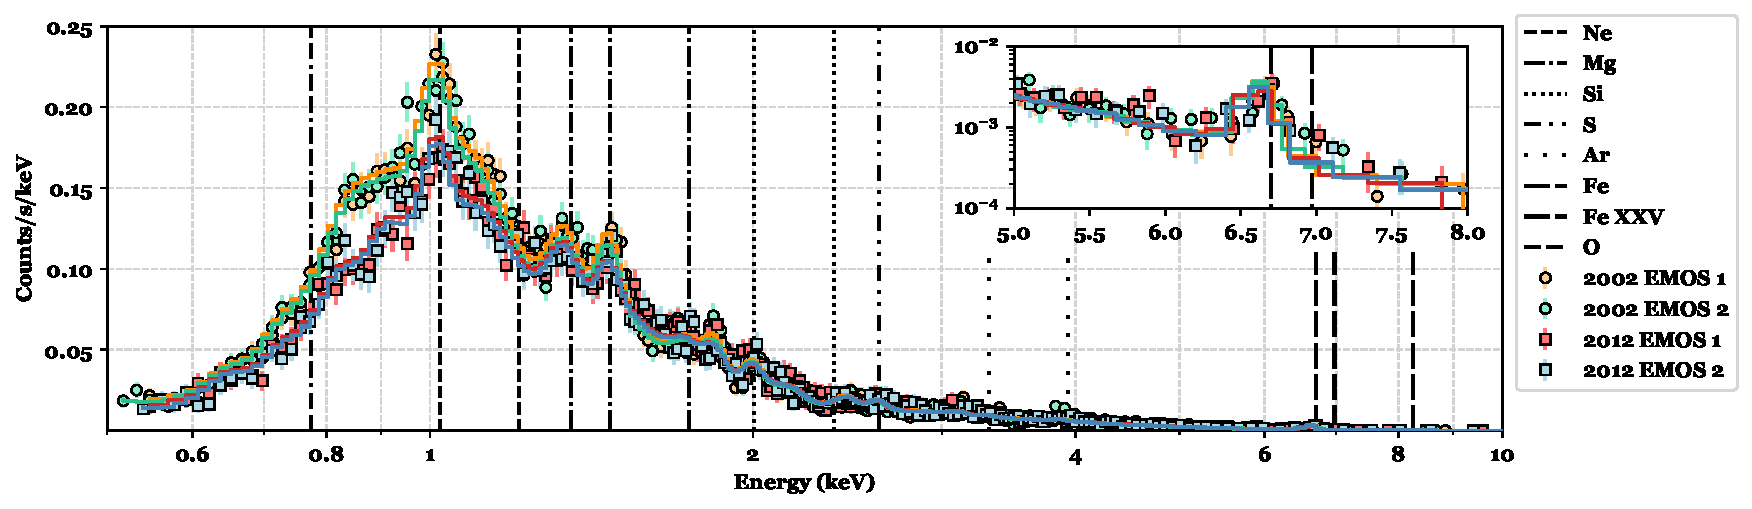
\includegraphics[width=0.95\linewidth]{Figures/SU Aur/figure_global_fit_energy.pdf}
    \caption{SU Aur. The best fit model to the 2002 and 2012 EMOS \& EPN data. Wavelengths of significant atomic species emission lines are shown with dashed/dotted lines.}
    \label{fig:su_aur_fit}
\end{figure*}

% How do my quiescent 2002 results compare to the ones from Robrade et al. '06 and Francosini et al. '07?
\citet{robrade_xmm-newton_2006} use a single absorbing component with three temperature components. Given that the emission measure is concentrated in the hottest component, it is not surprising that their $N\_{\mathrm{H}}$ value is similar to what we see in the hot component.
We see differences in the abundances and temperatures listed compared to our fits, at least partially due to the updated APEC models available today and our choice of a more modern set of nominal solar abundances.

\citet{franciosini_xmm-newton_2007} also use a single absorbing component with three temperature components.
They find a quiescent absorbing column density of $0.334\times10^{22} /cm^{-2}$, which is between the two absorbing component column densities that we find. 
The coolest temperature component found by them matches our coolest temperature component, but the two hotter components are cooler in our fit than in their fit. Again, their solar abundance \citep{anders_abundances_1989} differs from our choice \citep{asplund_chemical_2009}.

% - - - - - - - - - - - - - - - - - - - - - - - - - - - - - - - - - - - - - - - - - - - - 
\textit{Elemental Abundances}\label{sec:su_aur_abundance}

We also fit individual lines to determine the photon flux in the Lyman $\alpha$ and $\beta$ lines for several elements. The results are listed in Table \ref{table:line_fits}.

\begin{table}[t]
    \centering
    \begin{tabular}{|c|c|c|c|c|c|}
    \hline
    Line ID & $\lambda$ (\AA) & \multicolumn{2}{c|}{Flux (photons)}\\
    \hline
                   &       & 2002 & 2012  \\
    \hline
    O Ly $\alpha$  & 18.97 & $64.6 \pm 19.8$  &  $32.2 ± 16.2$ \\  % fine
    O Ly $\beta$   & 16.00 & $94.7 \pm 17.1$  &  $51.7 \pm 19.8$ \\ % fine
    Ne Ly $\alpha$ & 12.13 & $147.4 \pm 42.5$ & $129.6 \pm 45.7$ \\
    Ne Ly $\beta$  & 10.24 & $ 39.7 \pm 27.0$ &  $47.8 \pm 22.4$ \\
    Mg Ly $\alpha$ &  8.42 & $45.4 \pm 21.3$ &  $21.4 \pm 20.0$ \\ % fine
    Mg Ly $\beta$  &  7.11 & $32.1 \pm 18.1$ &  $0.0 \pm 16.3$ \\ % fine
    Si Ly $\alpha$ &  6.18 & $89.9 \pm 18.7$ &  $13.6 \pm 24.9$ \\ % fine
    \hline   
    \end{tabular}
    \caption{Measured line fluxes.}
    \label{table:line_fits}
\end{table}

% - - - - - - - - - - - - - - - - - - - - - - - - - - - - - - - - - - - - - - - - - - - - 
\subsubsection{Flare Properties}\label{sec:su_aur_flare}
For each of the epochs we divided the spectral data into quiescent and flaring periods, as described in Section \ref{sec:observations}, and separately fit the global plasma properties. We fit the flares using the same plasma model and procedure as the quiescent data, with one change due to the lower length and counts of the flaring spectrum.
At longer wavelengths ($\lambda > 17\;$\AA{}) the signal is much lower, yet this region includes the crucial oxygen emission lines. As above, \red{we fix the Oxygen abundance to solar}. All other parameters are fit, following the same procedure as the quiescent data.

\paragraph{2002 Flare}
The 2002 observations include three high flux events, centered around MJD's $52173.22, 52173.68$, and $52174.15$. Of the three events, the first is the brightest and the only one we analyse separately.
\citet{robrade_xmm-newton_2006}  found no significant abundance changes and no significant temperature changes. They found an increased emission level for all three temperature components, with the largest increase on the hottest component.
Similarly, \citet{franciosini_xmm-newton_2007} found no changes in abundance or absorption column density. They found increases in the temperature and emission measure of the two hotter components, while the cooler component stayed the same.
% What do i find?
We find consistent values for the absorbing column densities and abundances between the quiescent and flaring spectra. 
We also find that the middle temperature component has a much higher emission measure during the flare. The other two components have slightly higher emission measures. With the increase, the middle component has a higher emission measure than the high temperature component. In the quiescent spectrum, the ratios between the emission measures are: $EM_2/EM_1 \approx 0.91$ and $EM_3/EM_1 \approx 2.4$. In the flaring spectrum those change to: $EM_2/EM_1 \approx 3.1$ and $EM_3/EM_1 \approx 2.4$. 
The flare has peak temperatures of almost $70 MK$, compared to only $35 MK$ in the quiescent stage. Overall, our results align well with the results from \citet{franciosini_xmm-newton_2007}, with changes only in the temperatures and emission measures.

\textit{2012 Flare}
A flare was observed at the very end of Obs 0671960101 such that the rise and peak of the flare were recorded by the EPIC MOS and PN. The flare was not observed in the OM, since the OM was only operational during the first half of the observation.

% Plasma fit results
The results of the global plasma fit to the 2012 flare spectrum are listed in Table \ref{table:su_aur_fit}.
\red{The Ne abundance is similar to the quiescent. Magnesium, and Si are suggestively but not conclusively higher, and the Fe is significantly higher than in the quiescent data.}
We also find some changes in the temperatures and emission measures of the flare.
While the coolest temperature component and the middle temperature component are consistent, the hottest component is significantly hotter, with a temperature of $47.3 MK$, as compared to the quiescent $33.5 MK$. We also find that during the flare the first and second component EM decreases, and the third increases, changing the ratios to: $EM_2/EM_1\approx1.3$, and $EM_3/EM_1\approx5.9$. 

\begin{figure}
    \centering
    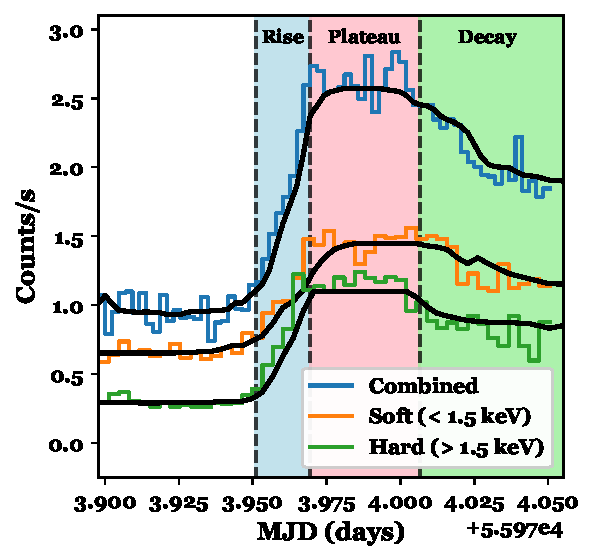
\includegraphics[width=0.9\linewidth]{Figures/SU Aur/figure_flare.pdf}
    \caption{Lightcurve of the flare, binned to 200s intervals. The combined, soft, and hard lightcurves are plotted in blue, orange, and green, respectively. Each is overplotted with a running median curve in black. The rise, plateau and decay phases of the flare are highlighted. The rise phase lasts for $0.444$ hours, and the plateau for $0.889$ hours.}
    \label{fig:su_aur_flare}
\end{figure}

% Flare morphology
Since the flare occurs at the end of the observing period the full decay of the flare is not fully observed and we are limited in our ability to analyze the flare duration and morphology. We identified three distinct phases in the flare morphology, a rise, plateau, and decay. We defined the rise as beginning when the count rate surpasses $1.1$ counts/s for 2 subsequent bins, and ending when it surpasses $2.5$ counts/s for 2 subsequent bins. Similarly, we define the plateau phase as beginning when the count rate surpasses $2.5$ counts/s for 2 subsequent bins and ends when it falls below $2.5$ counts/s for 2 bins. The decay phase begins when the plateau phase ends and is not fully captured by the observation. The rise phase lasts for $0.444$ hours, and the plateau for $0.889$ hours. The decay phase, while not completely observed, has a duration of at least $1.167$ hours.
% I don't know if this is actually a good way to do this.
% Also, am I sure the plateau is real?

With a plateau longer than the rise, the flare has a ``flat top" morphology, similar to that observed in several T Tauri stars in Orion by \citet{getman_x-ray_2008}. However, the ``slow-rise flat top" flares observed by \citet{getman_x-ray_2008}, demonstrated a much longer rise phase than shown here, with a typical duration of $12$ hours. 

\subsubsection{H$\alpha$ Emission} \label{sec:su_aur_halpha}
% Intro paragraph - What is the connection between young, active stars and Halpha emission? What other studies have observed double-peaked variable Halpha? Where does the shape and variability come from? What have previous studies of SU Aur Halpha found?
\halpha{} emission, caused by magnetic heating of the stellar chromosphere \citesomething{} has long been an important optical tracer of magnetic accretion \citesomething{}. 
Variable, double-peaked \halpha profiles have been observed for young stars and are attributed to changes in the accretion and disk wind \citep[e.g.][]{edwards_spectroscopic_1994, olson_rapid_1995, reipurth_halpha_1996, kurosawa_formation_2006}.
The \halpha variability of SU Aur was extensively monitored by \citet{giampapa_synoptic_1993} over a four-year time period. They found that the \halpha profile varied on timescales of days, and that the variation of the blue wing of \halpha{} was periodic with a period of $\sim2.98$days, in line with the stellar rotation.

% Paragraph describing our results & comparing to prior results
We see similar variability in the \halpha{} profile and equivalent width over a timescale of days (shown in Figure \ref{fig:halpha} and listed in Table \ref{table:ha_obs}). The EW(\halpha) starts at a maximum of $9.4$\AA, and decreases over seven days to a minimum of $\sim1.5$\AA, before increasing again.
\red{The decrease in the EW(\halpha) is caused by the increased self-absorption over that time period. At the minimum EW the center of the line is strongly absorbed, with emission only in the wings.}
Unlike \citet{giampapa_synoptic_1993}, we do not observe any periodicity in the EW signal over the $9$ days of observations. % Periodigram is not super helpful since it's 12 data points, but the peak signal is from the daily observations & aliases, not any data signal

% Profile changes
Starts at a somewhat asymmetric profile, with Reipurth Type III \citep{reipurth_halpha_1996}, the profile then shifts over the seven day period to become nearly fully symmetric (Reipurth Type II), and then the red wing starts increasing again. 

Simultaneously the amount of absorption increases. The central dip starts relatively small and increases until it is sub-continuum in Observation 7, continuing to increase through observations 10 \& 11, and then decreasing. \red{This could also be moved into the discussion section} The X-ray observations fall roughly in the middle of the \halpha{} observing period, when the central self-absorption is strongest. In the X-ray fits, the presence of the cool accretion component is unconstrained, compatible with either the absence of soft, accretion-related emission, or a high-absorbing column density that absorbs all soft emission that that it is not observable to us (and thus cannot be constrained in the fit). The \halpha{} line profile points to the second interpretation: The wide wings indicate an accretion rate of XXXXX and one interpretation of the central self-absorption is that the accretion spot on the star itself is covered by cooler, inflowing material. Of course, the formation of the \halpha{} in cTTS is complex with contributions from the disk and the wind as well, but at least this argument indicates that the the presence of a soft, but unseen, X-ray component from an accretion shock is likely during our X-ray observation.  

\begin{figure}[h]
    \centering
    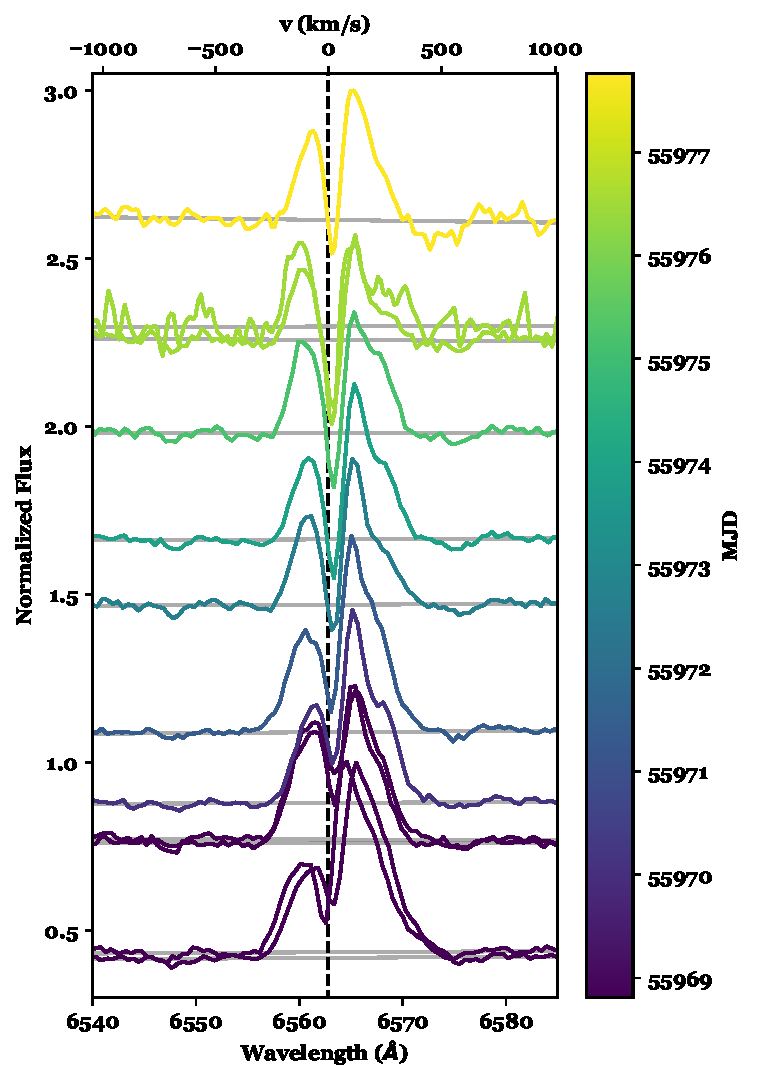
\includegraphics[width=0.9\linewidth]{Figures/SU Aur/figure_halpha.pdf}
    \caption{The \halpha{} region of our optical spectra. The wavelength and normalized flux of each spectrum is shown, with the vertical spacing and color according to the time. The psuedo-continuum for each spectrum is underplotted in gray. The \halpha{} profile changes significantly over the $9$ days covered by the observations, with increasing self-absorption, and a changing ratio of red-wing to blue-wing flux.}
    \label{fig:halpha}
\end{figure}

\begin{table*}[]
    \centering
    \begin{tabular}{|c|c|c|c|c|c|}
        \hline
         Obs Number & MJD & Telescope/Instrument & EW(\halpha) & EW blue wing & EW red wing \\
         & days & & \AA & \AA & \AA \\
         \hline
         1  & 55968.80775 & LHIRES III 600 l/mm  & 9.43 & 2.60 & 6.47 \\
         2  & 55968.81889 & LHIRES III 1200 l/mm & 8.50 & 2.33 & 5.84 \\
         3  & 55969.76617 & LHIRES III 600 l/mm  & 5.94 & 2.59 & 3.24 \\
         4  & 55969.82418 & LHIRES III 1200 l/mm & 5.69 & 2.38 & 3.16 \\
         5  & 55970.84233 & LHIRES III 1200 l/mm & 7.70 & 2.29 & 5.07 \\
         6  & 55971.82925 & LHIRES III 1200 l/mm & 8.33 & 2.68 & 5.45 \\
         7  & 55972.84902 & LHIRES III 1200 l/mm & 3.83 & 1.34 & 2.43 \\
         8  & 55973.84755 & LHIRES III 1200 l/mm & 4.26 & 1.28 & 2.96 \\
         9  & 55974.80521 & LHIRES III 1200 l/mm & 3.13 & 1.16 & 2.02 \\
         10 & 55975.75699 & LHIRES III 600 l/mm  & 1.61 & 0.75 & 0.92 \\
         11 & 55975.83785 & LHIRES III 1200 l/mm & 1.54 & 0.71 & 0.97 \\
         12 & 55977.76285 & LHIRES III 600 l/mm  & 3.00 & 1.03 & 1.95 \\
         \hline
    \end{tabular}
    \caption{\halpha{} observations and EW measurements.}
    \label{table:ha_obs}
\end{table*}

% - - - - - - - - - - - - - - - - - - - - - - - - - - - - - - - - - - - - - - - - - - - - - 
% - - - - - - - - - - - - - - - - - - - - - - - - - - - - - - - - - - - - - - - - - - - - - 

\subsection{AB Aur} \label{sec:ab_aur}
\subsubsection{X-Ray Lightcurve}

The X-Ray lightcurves from both the 2002 and 2012 epochs are shown in Figure \ref{fig:ab_aur_lc}. 
\citet{stelzer_statistical_2007} and \citet{telleschi_first_2007} found that the X-ray light curve is variable with a period of $\sim42$ hours. We fit a sine curve to the lightcurve and recover a period of $42$ hours. Using a smaller binning of $1.2$ks, we recover a slightly longer, but consistent period of 48 hours.

In the 2012 lightcurve we find no evidence for a periodic signal. With either the 5ks or 1.2ks binned data, the best-fit sine curve has period more than $6$ times longer than the observations, and is a worse statistical fit (according to a $\chi^2$ test) than a linear model.

% UPDATED 2024-10-22
\begin{figure*}
    \centering
    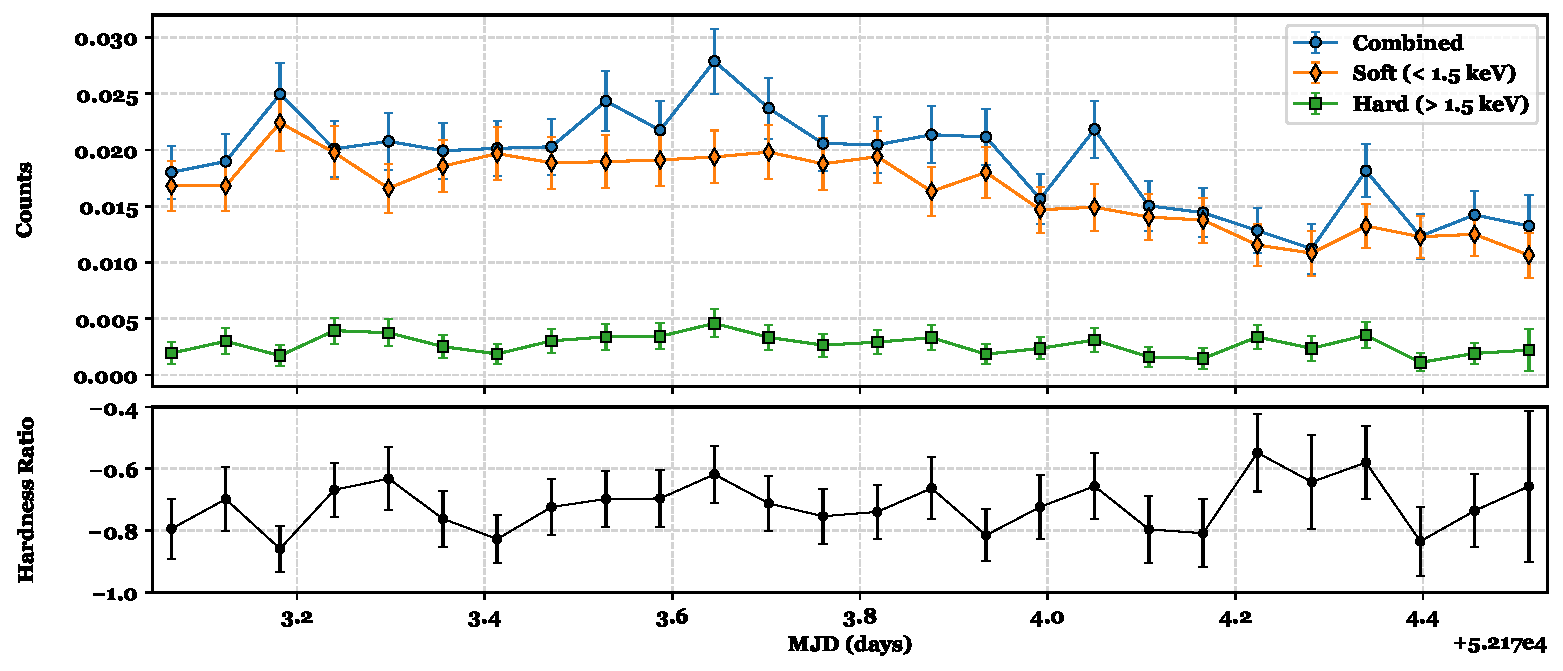
\includegraphics[width=0.85\linewidth]{Figures/AB Aur/figure_2002_lc_5000.pdf}
    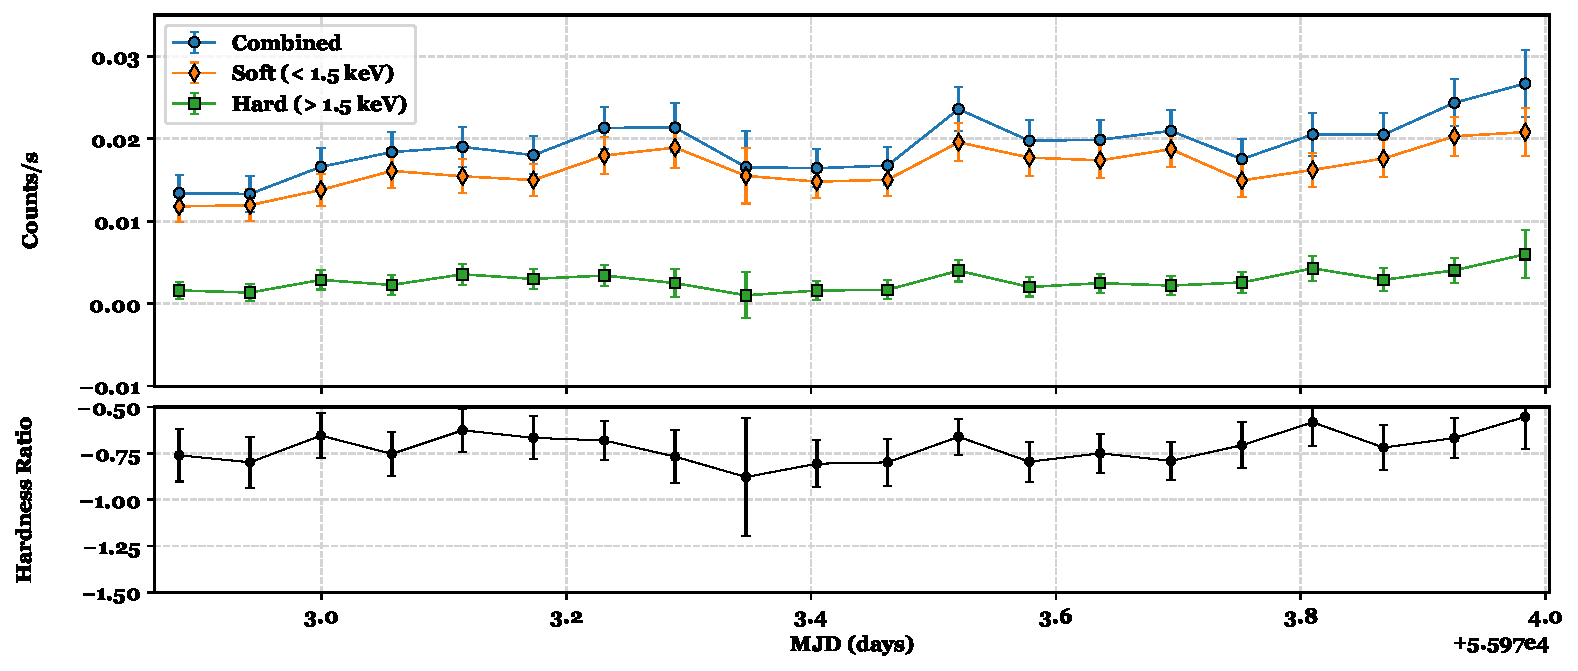
\includegraphics[width=0.85\linewidth]{Figures/AB Aur/figure_2012_lc_5000.pdf}
    \caption{Top) EPIC LC's and hardness ratio for 2002 data, binned to 5,000s intervals. Bottom) EPIC LC's and hardness ratio for 2012 data, binned to 5,000s intervals. In both, the combined, soft, and hard LC's are shown in blue circles, orange diamonds, and green squares respectively. AB Aur did not flare during either observation.}
    \label{fig:ab_aur_lc}
\end{figure*}

\subsubsection{Plasma Properties}

We determined the plasma properties of AB Aur by fitting the EMOS spectra, as described in Section \ref{sec:plasma}.

% - - - - - - - - - - - - - - - - - - - - - - - - - - - - - 
\textit{Global Fit}

We performed a global fit to the EMOS spectra using a model with a single absorption component and two temperature components, following \citet{telleschi_first_2007}. We also tested more complex models, but found that there was no evidence to support them over the simpler model, using a $\chi^2$ test. The resulting fit is shown in Figure \ref{fig:ab_aur_fit}, and listed in Table \ref{table:ab_aur_fit}. 

% UPDATED 2024-10-22
\begin{table}
\begin{tabular}{|c|c|c|}
\hline
Parameter & 2002 & 2012 \\
\hline
$N_{H_1}(10^{22} cm^{-2})$  & $0.029 \pm \inf $     & $0.226 \pm \inf$  \\
C, N, O (fixed)             & $1.0$                 & $1.0$             \\
Ne                          & $0.3 \pm 0.22$        & $0.5 \pm 0.25$ \\
Mg, Ni, Si, Fe, Ca, Al      & $0.2 \pm 0.03$        & $0.2 \pm 0.03$   \\
% Si                          & $0.3 \pm 0.103$     & $0.231\pm0.136$   \\
% Fe, Ca, Al                  & $0.2 \pm 0.022$           & $0.244 \pm\inf$   \\
$T_1 (10^6 K)$              & $2.2 \pm \inf$        & $2.3 \pm 0.1$    \\
$T_2 (10^6 K)$              & $9.2 \pm 0.2$         & $8.9 \pm 0.4$    \\
$EM_1 (10^{52} cm^{-3})$    & $0.073 \pm \inf $     & $0.064\pm\inf$    \\
$EM_2 (10^{52} cm^{-3})$    & $0.386 \pm 0.026$     & $0.249\pm0.025$   \\
% - - - - - - - - - - - - - - - - - - - - - - - - - - - - -
\hline
$\chi^2$        & $94.03$ & $160.976$ \\
Red. $\chi^2$   & $0.839$ & $0.752$  \\
D.o.F.          & $112$   & $214$    \\
\hline
\end{tabular}
\label{table:ab_aur_fit}
\caption{Global Fit results for AB Aur.}
\end{table}

% UPDATED 2024-10-22
\begin{figure*}
    \centering
    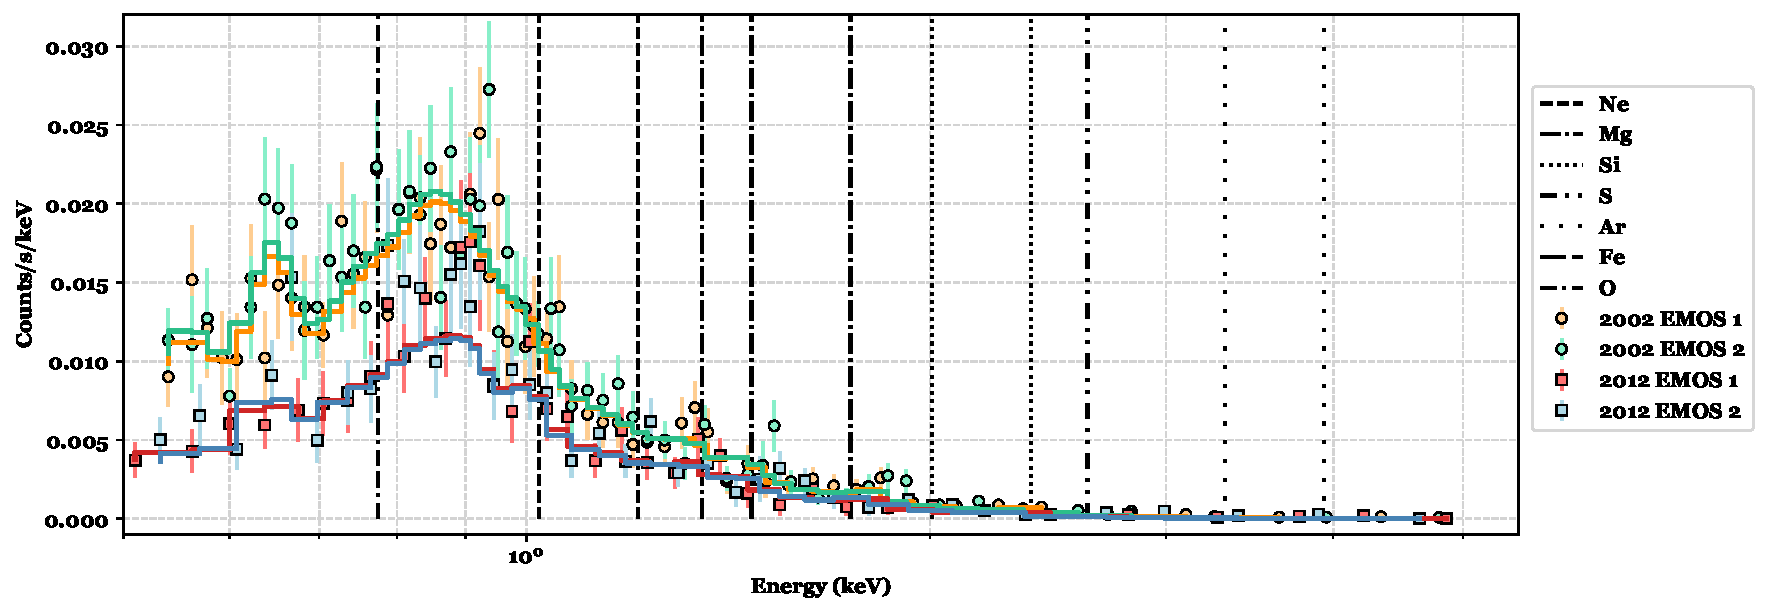
\includegraphics[width=0.85\linewidth]{Figures/AB Aur/figure_global_fit_energy.pdf}
    \caption{Global fit to EMOS and EPN data for the 2002 and 2012 data. Wavelengths of significant emission lines are marked with vertical lines.}
    \label{fig:ab_aur_fit}
\end{figure*}

We find that the temperatures, elemental abundances, absorbing column densities and emission measures are consistent between the two epochs at the $3\sigma$ level. 

% - - - - - - - - - - - - - - - - - - - - - - - - - - - - - - - - - - - - - - - - - - - - - 
% - - - - - - - - - - - - - - - - - - - - - - - - - - - - - - - - - - - - - - - - - - - - - 
\section{Summary and Discussion}\label{sec:discussion}

\subsection{SU Aur}

% The Model
For the T Tauri star SU Aur we find that a model with two absorption components and three temperature components produces the best statistical fit to the data. \red{\textbf{However, the differences in the resulting model fit from other, simpler, models is negligible.} Considering systematic uncertainties on the spectrum, it is not possible to say that the two absorption component model is definitively supported by the data.} 

However, the fit is still suggestive of the structure of SU Aur, indicating that there is \red{a region of plasma} with a higher absorbing density and two lower temperature components, and a second with a lower absorbing density and single, hotter temperature component. The second region, which is hot and low-density, is consistent with a stellar coronae, as would be expected for a T Tauri star like SU Aur, and has been found by previous studies \citesomething{}. The first region is consistent with an accretion column \citesomething{}, which has not been previously observed for SU Aur \citesomething{}. 
In particular, the two temperature components tied to the higher absorbing density plasma, suggests that the accretion column may have a complex, stratified structure, as suggested for T Tau \citep{schneider_multiepoch_2018}. 

% Stability
- The plasma properties from 2012 are all consistent with the results from 2002, suggesting a large-scale stability in the corona \& accretion shock over a ten year period of time
- The changes in the \halpha{} profile and EW over a $\sim7$ day period suggest short-term variability in the accretion

\newpage{}
\begin{acknowledgments}

\end{acknowledgments}

%% To help institutions obtain information on the effectiveness of their telescopes the AAS Journals has created a group of keywords for telescope facilities.
%
%% Following the acknowledgments section, use the following syntax and the
%% \facility{} or \facilities{} macros to list the keywords of facilities used 
%% in the research for the paper.  Each keyword is check against the master 
%% list during copy editing.  Individual instruments can be provided in 
%% parentheses, after the keyword, but they are not verified.

\vspace{5mm}
\facilities{\xmm{}, }

%% Similar to \facility{}, there is the optional \software command to allow 
%% authors a place to specify which programs were used during the creation of 
%% the manuscript. Authors should list each code and include either a
%% citation or url to the code inside ()s when available.

\software{XMM SAS, Sherpa, CIAO 4.15, ChiantiPy, astropy, numpy, matplotlib}


\bibliography{bib}{}
\bibliographystyle{aasjournal}

\end{document}
